\documentclass[10pt,a4paper]{article}

\usepackage{graphicx}
\usepackage{xcolor}
\usepackage{geometry}
\usepackage{amsmath}
\usepackage{booktabs}
\usepackage{tabularx}
\usepackage{adjustbox}
\usepackage{enumitem}
\usepackage{caption}
\usepackage{tikz}
\usetikzlibrary{arrows.meta,positioning}

% hyperref - ALWAYS last among content packages
\usepackage[
  colorlinks=true,
  linkcolor=blue!60!black,
  citecolor=gray!30!black,
  urlcolor=blue!60!black,
  bookmarks=true,
  bookmarksnumbered=true,
  unicode=true
]{hyperref}

\geometry{a4paper, top=2.3cm, bottom=2.3cm, left=2.3cm, right=2.3cm}

% float packing: avoid half-empty pages caused by deferred floats
\renewcommand{\topfraction}{0.95}
\renewcommand{\bottomfraction}{0.8}
\renewcommand{\textfraction}{0.05}
\renewcommand{\floatpagefraction}{0.85}
\setlength{\textfloatsep}{10pt plus 2pt minus 2pt}
\setlength{\intextsep}{10pt plus 2pt minus 2pt}

\usepackage[numbers,sort&compress]{natbib}
\bibliographystyle{unsrtnat}

\widowpenalty=10000
\clubpenalty=10000
\setlength{\emergencystretch}{1.5em}

\captionsetup{font=small,labelfont=bf,skip=5pt}

\hypersetup{
  pdftitle={AI-Based Smart Electricity Consumption Prediction and Anomaly Detection: A Benchmark Study and Deployable Web System},
  pdfauthor={MD Tamim Hossen, Md Emon Sarkar, MD. Montasir Hasan, MD. Sheratul Muntahar Ratul, Afrina Nisha},
  pdfsubject={Smart energy, load forecasting, anomaly detection, machine learning},
  pdfkeywords={load forecasting, anomaly detection, XGBoost, LSTM, smart meter, energy analytics}
}

\begin{document}

% ============================================================ title block
\begin{center}
  {\LARGE\bfseries AI-Based Smart Electricity Consumption Prediction\\[2pt]
   and Anomaly Detection:\\[6pt]
   \large A Benchmark Study and Deployable Web System on Four Years of\\
   Household Meter Data\par}
  \vspace{14pt}
  {\normalsize
  MD Tamim Hossen, Md Emon Sarkar, MD. Montasir Hasan,\\
  MD. Sheratul Muntahar Ratul, Afrina Nisha\par}
  \vspace{5pt}
  {\small Department of Computer Science and Engineering\\
  Dhaka International University, Dhaka, Bangladesh\par}
  \vspace{5pt}
  {\small\itshape Supervisor: Paritosh Chandra Ray, Lecturer, Department of CSE,\\
  Dhaka International University\par}
  \vspace{2pt}
  {\small November 2026\par}
\end{center}
\vspace{6pt}

\noindent\rule{\textwidth}{0.4pt}
\begin{center}
\begin{minipage}{0.92\textwidth}
\small
\textbf{Abstract---}This paper presents an end-to-end artificial intelligence system for
short-term electricity consumption prediction and anomaly detection at the individual
household level. We benchmark eight forecasting models---two seasonal-na\"ive baselines,
Ridge regression, Holt--Winters exponential smoothing, Random Forest, XGBoost, LightGBM,
and a direct multi-step long short-term memory (LSTM) network---on the UCI Individual
Household Electric Power Consumption dataset (2.08 million minute-level readings,
December 2006 to November 2010), under a strict day-ahead evaluation protocol in which
every feature available to a model is at least 24 hours old. Gradient-boosted trees
prove the strongest family: XGBoost attains a test RMSE of 0.588\,kW, a 22.4\%
improvement over the seasonal-na\"ive baseline, with the LSTM competitive at 0.592\,kW
and the lowest MAE and MAPE. For anomaly detection we compare four
approaches---forecast-residual z-scoring, Isolation Forest, One-Class SVM, and an LSTM
autoencoder---on a controlled benchmark with 112 injected anomalies spanning spikes,
level shifts, and dropouts. The residual method dominates (ROC-AUC 0.885, F1 0.482),
and the per-type analysis exposes a sharp asymmetry: spikes are detected with
93--98\% recall, whereas near-zero dropout events largely evade every tested detector.
A case study on the unmodified test period surfaces plausible real anomalies, including
multi-hour evening consumption excursions exceeding 4\,kW. Finally, we package the
selected models behind a Flask web service with an interactive dashboard and a REST
API, deployable to the Render platform, closing the loop from data to an operational
decision-support tool. All code, trained models, figures, and the training notebook are
released publicly.

\vspace{4pt}
\textbf{Keywords---}load forecasting; anomaly detection; XGBoost; LSTM; autoencoder;
smart meter; time series; deployed machine learning
\end{minipage}
\end{center}
\noindent\rule{\textwidth}{0.4pt}
\vspace{6pt}

% ============================================================ 1
\section{Introduction}\label{sec:intro}

Electricity is consumed the instant it is produced, so every actor in the power
value chain---from grid operators balancing frequency to retailers pricing tariffs and
households sizing rooftop solar and batteries---benefits from knowing consumption in
advance. The same household meter stream enables a second, complementary capability:
detecting when consumption behaves abnormally. Abnormal patterns can indicate a failing appliance left running, an inefficient
device drawing standby power, or simply an unexpected change in occupancy that
invalidates existing schedules and contracts.
Forecasting and anomaly detection are therefore two sides of the same smart-metering
pipeline, and practical systems increasingly require both, delivered together and
evaluated on equal footing.

Household-level forecasting is, however, substantially harder than its aggregate
counterpart. System-level load is the convolution of thousands of consumers, and the
law of large numbers smooths individual behaviour into a series dominated by
calendar cycles and weather; predictive models routinely reach coefficients of
determination above 0.9 at the system level~\cite{alfares2002electric,hong2016probabilistic}.
A single household's hourly consumption instead reflects the stochastic timing of a
handful of appliance events---a kettle, a dryer, a water heater---superimposed on a
slowly varying baseline. The predictable component shrinks, and the irreducible noise
grows accordingly~\cite{kong2019lstm}. This raises a first question that this paper
addresses systematically: \emph{how much} of a household's next-day consumption is
actually predictable, and which model family captures it best?

A second question concerns anomaly detection methodology. Published evaluations of
smart-meter anomaly detectors differ widely in protocol, and several popular methods
are examined only on data whose anomalies are of a single, easy kind. We argue that a
fair comparison must (i) inject anomaly types of contrasting sign and duration---sharp
high-consumption spikes, sustained level shifts, and prolonged near-zero dropouts---and
(ii) contaminate the lagged features that detectors consume, rather than only the
evaluation target, so that the measured robustness reflects operational conditions.
Under this protocol we quantify how four standard detectors, spanning three distinct
paradigms, trade off against one another.

Third, machine-learning research on this problem often stops at metrics tables. To be
useful, a trained model must be reachable by non-specialists and by other software. We
therefore package the best-performing forecaster and the residual anomaly detector
into a lightweight web application with an interactive dashboard and a documented REST
API, deployable on a free-tier platform (Render), and we report the engineering
decisions that keep the service inside a 512\,MB memory budget.

The contributions of this work are:
\begin{enumerate}[leftmargin=1.6em,itemsep=1pt,topsep=2pt]
\item A controlled benchmark of eight forecasting models on four years of real
      household meter data under a \emph{strict} 24-hour-ahead protocol, with
      hyperparameters selected on a chronological validation split and all results
      reported on an untouched eight-month test period.
\item A contamination-aware anomaly detection study comparing residual z-scoring,
      Isolation Forest, One-Class SVM, and an LSTM autoencoder across three injected
      anomaly types, plus a case study of the strongest events found in the real,
      unmodified test data.
\item An analysis of where each approach fails: the asymmetry between easily detected
      high-consumption spikes and nearly invisible dropouts, and the evening-hour
      concentration of forecast errors.
\item A deployable web system (Flask, Chart.js, REST API, Render configuration) that
      serves day-ahead forecasts, live forecasts on user-supplied histories, anomaly
      scores, and the full benchmark leaderboard, together with the complete public
      repository of code, models, figures, and a reproducible Kaggle notebook.
\end{enumerate}

% ============================================================ 2
\section{Related Work}\label{sec:related}

Load forecasting is one of the oldest applications of statistical time-series
modelling. Alfares and Nazeeruddin~\cite{alfares2002electric} classify the
pre-machine-learning literature into regression, exponential smoothing, and
knowledge-based approaches; Hong and Fan~\cite{hong2016probabilistic} later survey the
shift toward probabilistic and data-driven methods. Classical exponential smoothing
with trend and seasonality originates with Winters~\cite{winters1960forecasting} and
remains a strong, assumption-light baseline that we include in our benchmark.
Seasonal-trend decomposition by loess (STL)~\cite{cleveland1990stl} provides the
standard lens for inspecting the calendar structure of demand series.

Within machine learning, tree ensembles and neural networks dominate recent practice.
Random Forests~\cite{breiman2001random} aggregate decorrelated decision trees and
handle mixed tabular features with little preprocessing. Gradient-boosted trees
refine the idea by sequentially fitting shallow trees to residual errors;
XGBoost~\cite{chen2016xgboost} popularised regularised, histogram-based implementations
that win a large share of tabular data competitions, and
LightGBM~\cite{ke2017lightgbm} accelerated training further with leaf-wise growth and
gradient-based one-side sampling. On the neural side, recurrent architectures were
designed specifically to retain long-range temporal context;
LSTM~\cite{hochreiter1997lstm} alleviates the vanishing-gradient problem of vanilla
recurrent networks and has become the reference deep architecture for
short-term load forecasting. Kong et al.~\cite{kong2019lstm} apply LSTM networks to
residential load at various horizons and find that, while deep models outperform
classical baselines, individual-customer load remains far less predictable than
aggregate load---an observation our results reproduce and quantify.

Anomaly detection methodology is surveyed by Chandola et
al.~\cite{chandola2009anomaly}, who classify approaches into statistical,
proximity-based, and one-class boundary methods. Isolation
Forest~\cite{liu2008isolation} detects outliers by random recursive partitioning,
exploiting the fact that anomalies isolate in fewer splits; its linear complexity
makes it a default choice for streaming features. The One-Class
SVM~\cite{scholkopf2001ocsvm} learns a boundary enclosing the bulk of a kernelised
density and flags points outside it. Reconstruction-based methods train a model to
rebuild normal patterns and treat reconstruction error as an anomaly score; Sakurada
and Yairi~\cite{sakurada2014autoencoder} demonstrated that autoencoders capture
nonlinear normality that linear PCA misses, establishing the recipe we adopt for our
LSTM autoencoder. In the energy domain, forecast-residual methods are attractive
because they reuse the forecaster already required by the system: the residual between
actual and predicted consumption is standardised, and large deviations are
flagged~\cite{hyndman2021fpp}. Our study compares all four families under a
feature-contaminating injection protocol with sign-diverse anomaly types on this
benchmark dataset, on equal footing with the forecasting task itself.

% ============================================================ 3
\section{Dataset and Exploratory Analysis}\label{sec:data}

\subsection{Source data}
We use the UCI Individual Household Electric Power Consumption
dataset~\cite{hebrail2012uci}, which records one household in Sceaux, France (7\,km
south of Paris), at one-minute resolution for 47 months (December 2006 to November
2010). The archive contains 2{,}075{,}259 rows and nine attributes: global active and
reactive power (kW), voltage (V), global intensity (A), and three appliance-group
sub-meterings (kitchen; laundry room; water heater and air conditioner, in
watt-hours). The household also owns unmetered loads, whose contribution is recoverable
as the residual of the global measurement and the sub-meters. Table~\ref{tab:data}
summarises the dataset and our processed splits.

\begin{table}[t]
\centering
\caption{Dataset summary and chronological splits (after cleaning).}
\label{tab:data}
\small
\begin{tabular*}{\textwidth}{@{\extracolsep{\fill}} l l l}
\toprule
\textbf{Property} & \textbf{Value} & \textbf{Notes} \\
\midrule
Raw rows (minute level) & 2{,}075{,}259 & 47 months, Dec 2006 -- Nov 2010 \\
Rows with missing values & 25{,}979 (1.25\%) & contiguous sensor outages \\
Rows after interpolation & 2{,}050{,}108 & linear-in-time, gaps $\le$ 60 min \\
Hourly rows after aggregation & 34{,}176 & mean of global active power (kW) \\
Hourly mean / std / max & 1.09 / 0.90 / 6.56 kW & \\
Daily energy (mean) & $\approx$ 26.1 kWh & \\
\midrule
Train split & 21{,}951 hours & 2006-12-23 -- 2009-06-30 \\
Validation split & 6{,}480 hours & 2009-07-01 -- 2010-03-31 \\
Test split & 5{,}554 hours & 2010-04-01 -- 2010-11-26 \\
\bottomrule
\end{tabular*}
\end{table}

\subsection{Preprocessing}
Minute-level rows containing missing values (1.25\% of the archive, occurring in
contiguous outages) were interpolated linearly in time with a 60-minute cap, and hours
with insufficient raw coverage were dropped. The cleaned series was aggregated to
hourly means of global active power, yielding 34{,}176 hourly observations. We
deliberately exclude instantaneous electrical covariates (voltage, intensity) from the
feature set: in a genuine day-ahead setting their future values are unknown, and
including them would leak contemporaneous information.

\subsection{Exploratory findings}
Figure~\ref{fig:overview}(a) shows daily energy over the full four years with the
chronological split boundaries. The series is stationary in the mean with no
long-term drift, but exhibits dense bursts of high-consumption days in winter
(heating-related loads) and occasional multi-day low-consumption troughs consistent
with absences. Figure~\ref{fig:overview}(b) contrasts average weekday and weekend
profiles: a sharp weekday morning ramp peaking near 07:00--08:00, an evening peak
around 18:00--20:00, and a flatter, delayed weekend morning. The mean hourly load is
1.09\,kW (about 26.1\,kWh per day).

\begin{figure}[t]
\centering
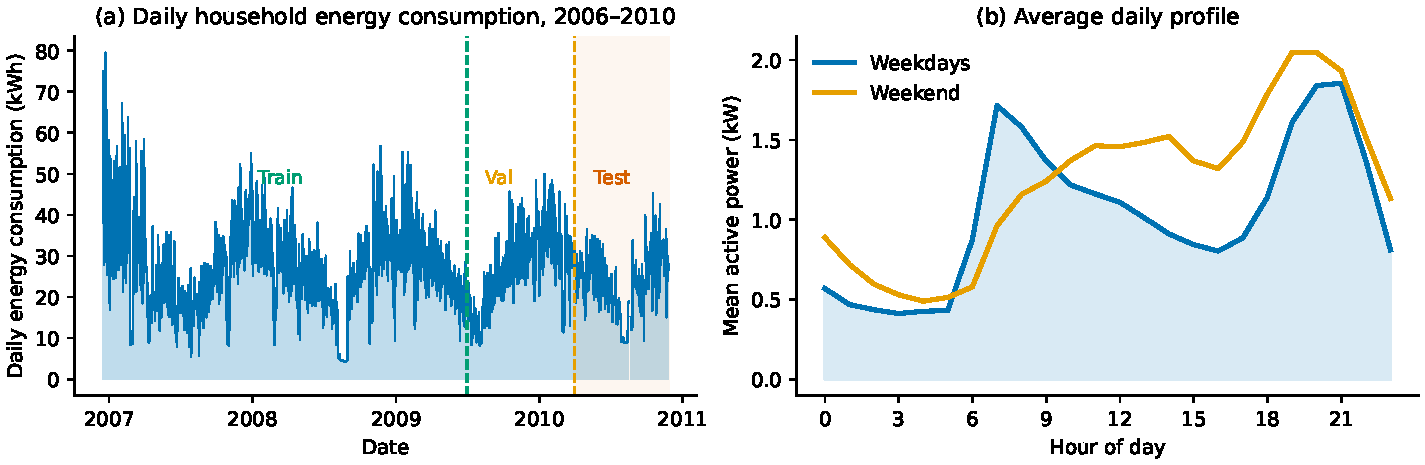
\includegraphics[width=0.9\textwidth]{../figures/fig1_dataset_overview.pdf}
\caption{Dataset overview. (a) Daily energy consumption with chronological
train/validation/test boundaries; (b) average daily profile, weekdays versus
weekend, showing the morning and evening ramps that motivate hour-of-day features.}
\label{fig:overview}
\end{figure}

Figure~\ref{fig:seasonality}(a) maps mean power by month and hour of day, revealing
strong daily periodicity in all months, elevated winter consumption, and the
double-peak structure of the daily profile. Figure~\ref{fig:seasonality}(b) applies
STL decomposition~\cite{cleveland1990stl} to a two-month window: the trend absorbs
slow weather-driven variation while the daily seasonal component captures the
recurring profile. These structures justify the lag and calendar features used by the
supervised models, and the residual component foreshadows the difficulty of the
day-ahead task: hour-to-hour movements of one to two kilowatts are routine.

\begin{figure}[t]
\centering
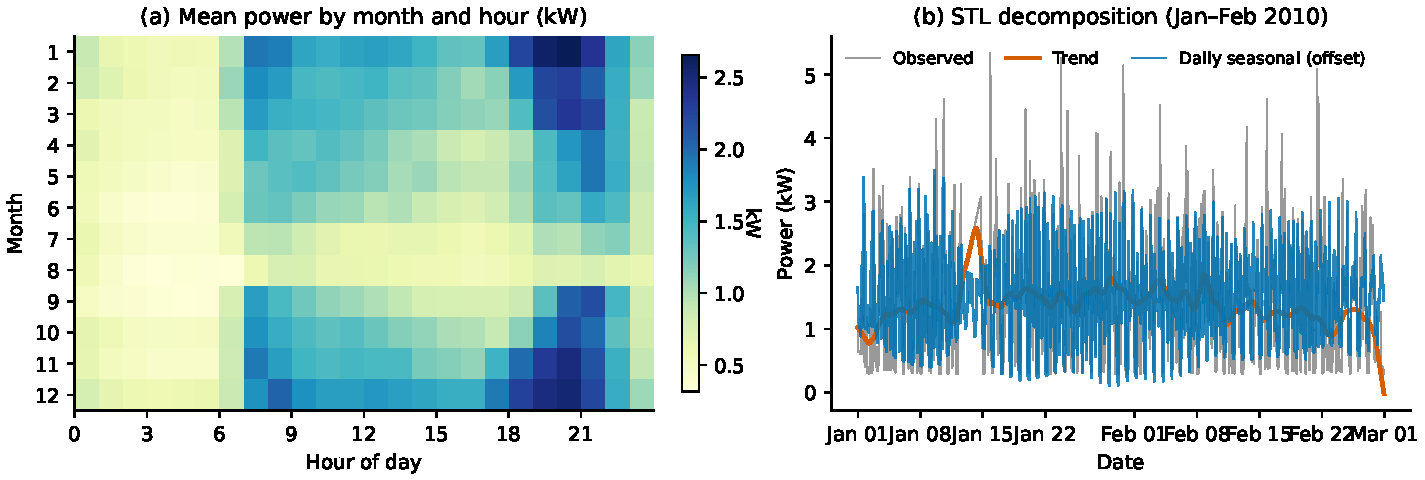
\includegraphics[width=0.9\textwidth]{../figures/fig2_seasonality.pdf}
\caption{Seasonality analysis. (a) Mean active power by month and hour of day;
(b) STL decomposition (period 24 h, robust) of January--February 2010 showing
observed, trend, and daily seasonal components.}
\label{fig:seasonality}
\end{figure}

% ============================================================ 4
\section{Methodology}\label{sec:method}

Figure~\ref{fig:arch} summarises the processing pipeline from raw data to the deployed
service. The remainder of this section details each stage.

\begin{figure}[t]
\centering
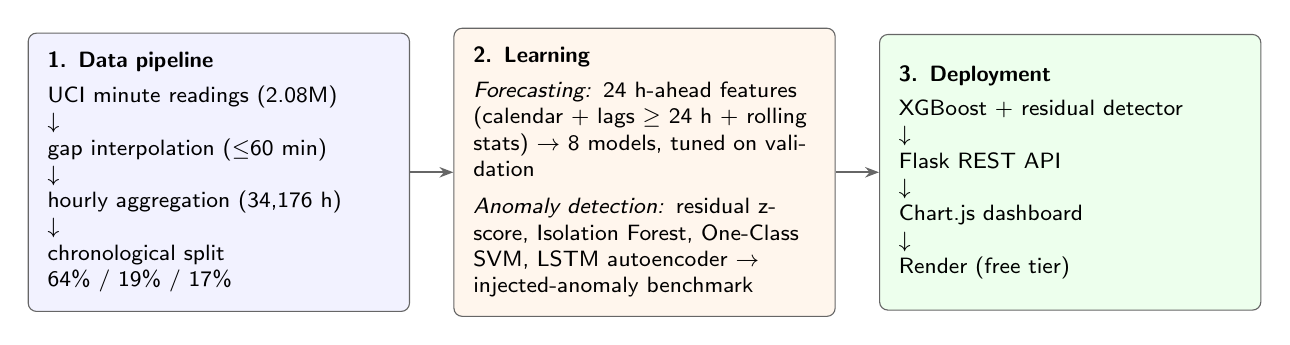
\begin{tikzpicture}[
  phase/.style={draw=black!60, rounded corners=3pt, text width=4.35cm,
                minimum height=3.5cm, align=left, font=\footnotesize\sffamily,
                inner sep=7pt},
  phasetitle/.style={font=\footnotesize\bfseries\sffamily},
  arr/.style={-{Stealth[length=5pt]}, thick, black!60}
]
\node[phase, fill=blue!5] (a) {%
  \textbf{1. Data pipeline}\\[3pt]
  UCI minute readings (2.08M)\\
  $\downarrow$\\
  gap interpolation ($\le$60 min)\\
  $\downarrow$\\
  hourly aggregation (34{,}176 h)\\
  $\downarrow$\\
  chronological split\\
  64\% / 19\% / 17\%};
\node[phase, fill=orange!7, right=0.55cm of a] (b) {%
  \textbf{2. Learning}\\[3pt]
  \emph{Forecasting:} 24 h-ahead features (calendar + lags $\ge$ 24 h + rolling
  stats) $\rightarrow$ 8 models, tuned on validation\\[4pt]
  \emph{Anomaly detection:} residual z-score, Isolation Forest, One-Class SVM,
  LSTM autoencoder $\rightarrow$ injected-anomaly benchmark};
\node[phase, fill=green!7, right=0.55cm of b] (c) {%
  \textbf{3. Deployment}\\[3pt]
  XGBoost + residual detector\\
  $\downarrow$\\
  Flask REST API\\
  $\downarrow$\\
  Chart.js dashboard\\
  $\downarrow$\\
  Render (free tier)};
\draw[arr] (a) -- (b);
\draw[arr] (b) -- (c);
\end{tikzpicture}
\caption{System architecture: data pipeline, learning stage, and deployment.}
\label{fig:arch}
\end{figure}

\subsection{Problem formulation}
Let $y_t$ denote the mean active power (kW) during hour $t$. The task is day-ahead
forecasting: at the end of day $d-1$, predict all 24 hourly values of day $d$.
Formally, for every target hour $t$ we seek an estimate
\begin{equation}\label{eq:task}
\hat{y}_t = f\!\left(\mathcal{F}_{<t-23\text{h}}\right),
\end{equation}
where the feature set $\mathcal{F}$ is restricted to information at least 24 hours
old. This is stricter than the common one-step-ahead protocol, which feeds the most
recent hour to the model, and it matches the operational day-ahead setting in which
schedules must be committed in advance.

\subsection{Feature engineering}
For each target hour $t$ we construct 11 features, all computed from data older than
$t-23$ hours:
\begin{itemize}[leftmargin=1.6em,itemsep=1pt,topsep=2pt]
\item \emph{Calendar:} hour of day, day of week, month, weekend indicator, day of
      year.
\item \emph{Autoregressive lags:} $y_{t-24}$, $y_{t-48}$, $y_{t-168}$ (same hour
      yesterday, two days ago, and one week ago).
\item \emph{Rolling statistics:} the mean and standard deviation of the 24 hours
      ending at $y_{t-24}$, and the mean of the 168 hours ending at $y_{t-24}$.
\end{itemize}
The lag-24 and lag-168 features encode the daily and weekly periodicity visible in
Figure~\ref{fig:seasonality}; the rolling statistics provide a local baseline level
that adapts to slow regime changes such as seasonal drift or occupancy shifts.

\subsection{Forecasting models}
Eight models of increasing capacity are compared; Table~\ref{tab:models} lists the
configuration selected for each on the validation split.
\begin{enumerate}[leftmargin=1.7em,itemsep=1pt,topsep=2pt]
\item \textbf{Seasonal na\"ive (24 h and 168 h):} $\hat{y}_t = y_{t-24}$ and
      $\hat{y}_t = y_{t-168}$. These require no training and define the skill
      baseline.
\item \textbf{Ridge regression:} linear model on cyclical (sine/cosine) encodings of
      hour, day of week, and month, plus the lag features; the $\ell_2$ penalty is
      selected on validation RMSE.
\item \textbf{Holt--Winters exponential smoothing:} additive trend with damping and
      daily seasonality (period 24), refit daily on a trailing eight-week window so
      that each day-ahead forecast uses only past data; additive and multiplicative
      seasonal variants are compared on validation.
\item \textbf{Random Forest~\cite{breiman2001random}:} 500 trees; depth and minimum
      leaf size selected on validation.
\item \textbf{XGBoost~\cite{chen2016xgboost}:} gradient-boosted trees with the
      histogram method, subsampling of rows and columns, and $\ell_2$ regularisation.
\item \textbf{LightGBM~\cite{ke2017lightgbm}:} leaf-wise growth with the same
      regularisation family.
\item \textbf{LSTM network~\cite{hochreiter1997lstm}:} a direct multi-step
      architecture that maps the past 168 hours (standardised consumption plus
      cyclical calendar channels) through a two-layer LSTM (hidden size 64) to all
      24 target hours at once, trained with Smooth-$L_1$ loss and early stopping on
      validation loss. For the day-ahead score reported in
      Table~\ref{tab:results}, hour $t$ is scored with the 24th output of the window
      ending 24 hours earlier---exactly the feature timeliness of
      Eq.~\eqref{eq:task}.
\end{enumerate}

\begin{table}[t]
\centering
\caption{Model configurations after validation-based selection.}
\label{tab:models}
\small
\begin{tabular*}{\textwidth}{@{\extracolsep{\fill}} l l l}
\toprule
\textbf{Model} & \textbf{Selected configuration} & \textbf{Final fit time} \\
\midrule
Seasonal na\"ive & none & -- \\
Ridge & $\alpha = 0.1$ (cyclical encoding) & $<$ 1 s \\
Holt--Winters & additive seasonal (24), damped trend, 8-week rolling refits & 171 s \\
Random Forest & 500 trees, max depth 18, min leaf 1 & 53 s \\
XGBoost & 800 trees, depth 4, learning rate 0.03 & 0.7 s \\
LightGBM & 800 trees, 31 leaves, learning rate 0.03 & 1.7 s \\
LSTM & 2 layers, hidden 64, horizon 24, early stop (epoch 6 of 40) & 336 s \\
\bottomrule
\end{tabular*}
\end{table}

\subsection{Anomaly detection framework}
We compare four detectors drawn from the statistical, density, boundary, and
reconstruction paradigms of unsupervised anomaly detection:
\begin{enumerate}[leftmargin=1.7em,itemsep=1pt,topsep=2pt]
\item \textbf{Residual z-score:} with the best forecaster $f$, the residual
  $r_t = y_t - \hat{y}_t$ is standardised by the residual standard deviation
  $\sigma$ estimated on the clean validation split,
  \begin{equation}\label{eq:zscore}
  z_t = \frac{\left|y_t - \hat{y}_t\right|}{\sigma}, \qquad
  \text{anomalous if } z_t > 3 .
  \end{equation}
\item \textbf{Isolation Forest~\cite{liu2008isolation}:} 300 trees on standardised
      consumption features (current value, lags, rolling statistics, calendar).
\item \textbf{One-Class SVM~\cite{scholkopf2001ocsvm}:} RBF kernel, $\nu$ matched to
      the expected contamination.
\item \textbf{LSTM autoencoder~\cite{sakurada2014autoencoder}:} a 24-hour window is
      encoded to a 32-unit vector and decoded back to 24 values; the per-hour
      anomaly score is the mean squared reconstruction error over all windows
      containing that hour, which localises scores better than the conventional
      window-end attribution.
\end{enumerate}

\subsection{Evaluation protocol}
Forecast quality is measured by RMSE, MAE, MAPE, and $R^2$ on the untouched test
split, together with the forecast skill score
\begin{equation}\label{eq:skill}
\text{Skill} = 1 - \frac{\mathrm{RMSE}}{\mathrm{RMSE}_{\text{naive-24h}}},
\end{equation}
the fractional RMSE improvement over the daily seasonal na\"ive baseline.

For anomaly detection, the dataset provides no ground-truth anomaly labels, so we
inject controlled anomalies into the \emph{test region only}: 112 anomalous hours
(2.02\% of test hours) comprising 44 single-hour spikes (consumption multiplied by
2.5--4.0 plus 1.5\,kW, capped at 8\,kW), 33 hours of level shifts (2--6 hour blocks
raised by 60--150\%), and 35 hours of dropouts (4--12 hour blocks forced to
0.02--0.10\,kW). Lag features are then \emph{recomputed from the contaminated
series}, so detectors must cope with polluted context exactly as they would in
operation. Detection quality is reported as precision, recall, and F1 at the
operating point matching the true prevalence (top-2\% of scores), plus threshold-free
ROC-AUC and PR-AUC, and recall is decomposed by anomaly type. A case study on the
clean, unmodified test period complements the synthetic benchmark.

% ============================================================ 5
\section{Results}\label{sec:results}

\subsection{Forecasting}
Table~\ref{tab:results} reports test-period performance for the strict day-ahead
task, and Figure~\ref{fig:comparison} visualises the ranking. Three families of
observations emerge.

\begin{table}[t]
\centering
\caption{Day-ahead (24 h) forecasting results on the test period
(Apr--Nov 2010, 5{,}554 hours). Best value per column in bold.}
\label{tab:results}
\small
\begin{tabular*}{\textwidth}{@{\extracolsep{\fill}} l r r r r r}
\toprule
\textbf{Model} & \textbf{RMSE (kW)} & \textbf{MAE (kW)} & \textbf{MAPE (\%)} &
\textbf{$R^2$} & \textbf{Skill (\%)} \\
\midrule
XGBoost           & \textbf{0.5875} & 0.4328 & 64.91 & \textbf{0.318} & \textbf{22.4} \\
LSTM              & 0.5920 & \textbf{0.4213} & \textbf{55.86} & 0.307 & 21.8 \\
LightGBM          & 0.5931 & 0.4354 & 65.93 & 0.304 & 21.6 \\
Random Forest     & 0.5937 & 0.4400 & 68.09 & 0.303 & 21.5 \\
Ridge             & 0.6060 & 0.4513 & 65.36 & 0.274 & 19.9 \\
Seasonal na\"ive (24 h)  & 0.7568 & 0.5101 & 65.97 & $-0.132$ & 0.0 \\
Holt--Winters     & 0.7860 & 0.5949 & 92.40 & $-0.222$ & $-3.9$ \\
Seasonal na\"ive (168 h) & 0.7948 & 0.5500 & 75.36 & $-0.249$ & $-5.0$ \\
\bottomrule
\end{tabular*}
\end{table}

\begin{figure}[t]
\centering
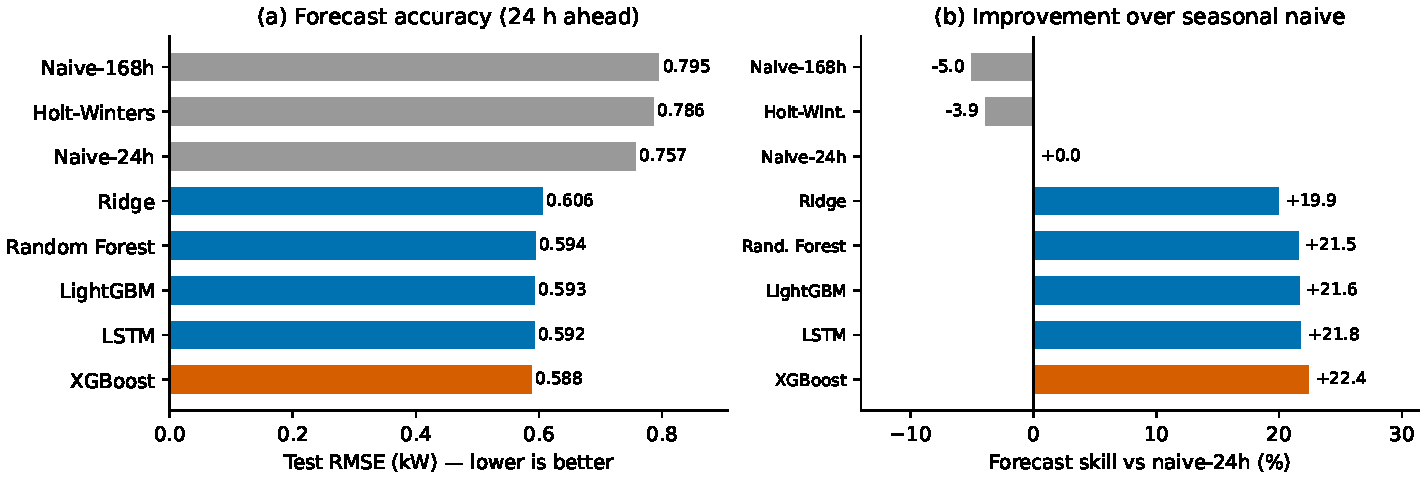
\includegraphics[width=0.9\textwidth]{../figures/fig3_model_comparison.pdf}
\caption{Forecast accuracy on the test period. (a) Test RMSE by model;
(b) forecast skill (Eq.~\eqref{eq:skill}) relative to the seasonal-na\"ive
24 h baseline. Red highlights the selected deployment model.}
\label{fig:comparison}
\end{figure}

First, \textbf{tree ensembles lead the ranking}. XGBoost achieves the best RMSE
(0.5875\,kW) and $R^2$ (0.318), a 22.4\% skill improvement over the seasonal
na\"ive---remarkable given that the baseline already exploits the strong daily
periodicity. LightGBM and Random Forest follow within 1\% of the leader, confirming
that the gradient-boosting advantage on tabular problems carries over to
day-ahead household load. The LSTM is statistically competitive on RMSE (0.5920\,kW)
and actually \emph{wins} on MAE (0.4213\,kW) and MAPE (55.9\%): the network errs
less on typical hours, while trees occasionally produce larger misses that RMSE
penalises quadratically. From a deployment standpoint the models are
interchangeable in accuracy; XGBoost is selected for its 0.7\,s final fit time,
small artefact size (0.8\,MB), and CPU-only inference.

Second, \textbf{the achievable $R^2$ is modest by aggregate-load standards}. A value
near 0.32 (versus $>$0.9 typical for system load) quantifies how much of a single
household's next-day hourly consumption is governed by unpredictable occupant
behaviour rather than calendar structure~\cite{kong2019lstm}. The MAPE values,
likewise high at 56--68\%, reflect the many near-zero overnight hours in which
relative errors blow up; MAE in kilowatts is the more interpretable scale here.

Third, \textbf{both na\"ive persistence and Holt--Winters underperform the mean}.
Holt--Winters trails even the 24-hour na\"ive baseline: the damped-trend
extrapolation of a rolling window adds noise on a series whose level wanders with
occupancy, and its 92\% MAPE illustrates how poorly an unregularised seasonal mean
tracks low-consumption hours. This is a useful caution against reaching for
classical smoothing as a default at the household level.

\begin{figure}[t]
\centering
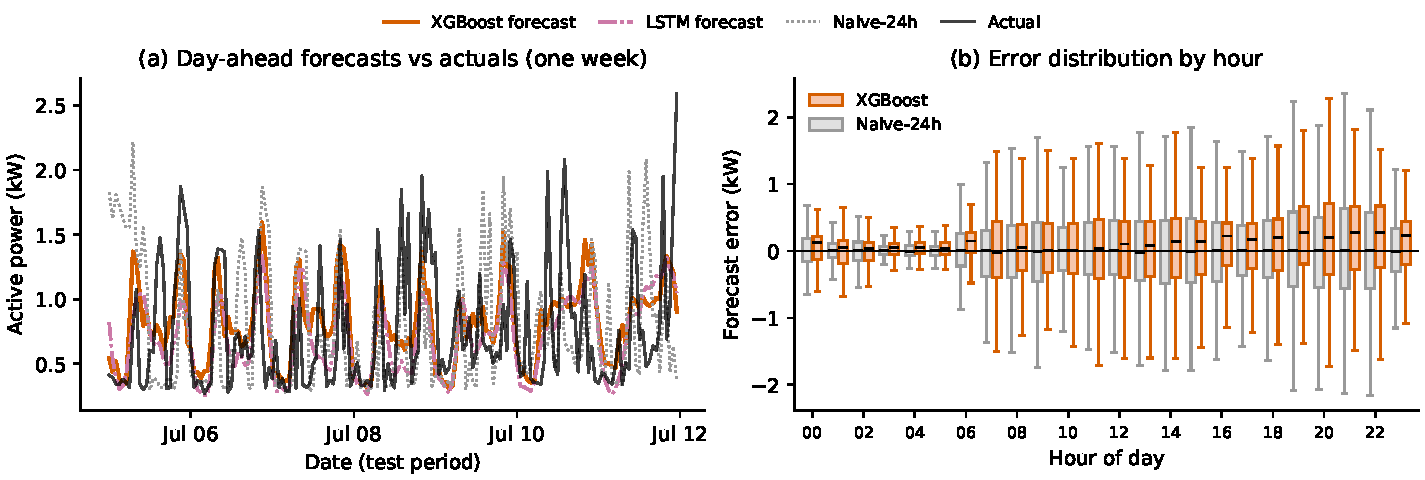
\includegraphics[width=0.9\textwidth]{../figures/fig4_forecast_quality.pdf}
\caption{Forecast behaviour on the test period. (a) One week of actual consumption
with day-ahead forecasts from XGBoost, LSTM, and the seasonal na\"ive;
(b) distribution of forecast errors by hour of day (XGBoost versus na\"ive-24 h),
showing the widest spread and largest positive bias during evening hours.}
\label{fig:quality}
\end{figure}

Figure~\ref{fig:quality}(a) illustrates a representative week: all models track the
daily shape, but evening peaks---where consumption is largest and most
behaviour-driven---attract the biggest errors. Panel (b) quantifies this: error
spread is widest between 17:00 and 22:00, where a drying cycle or a dinner with
guests can double the load relative to the previous day at the same hour. The na\"ive
baseline shows a systematic positive evening bias that the learned models largely
remove.

\begin{figure}[t]
\centering
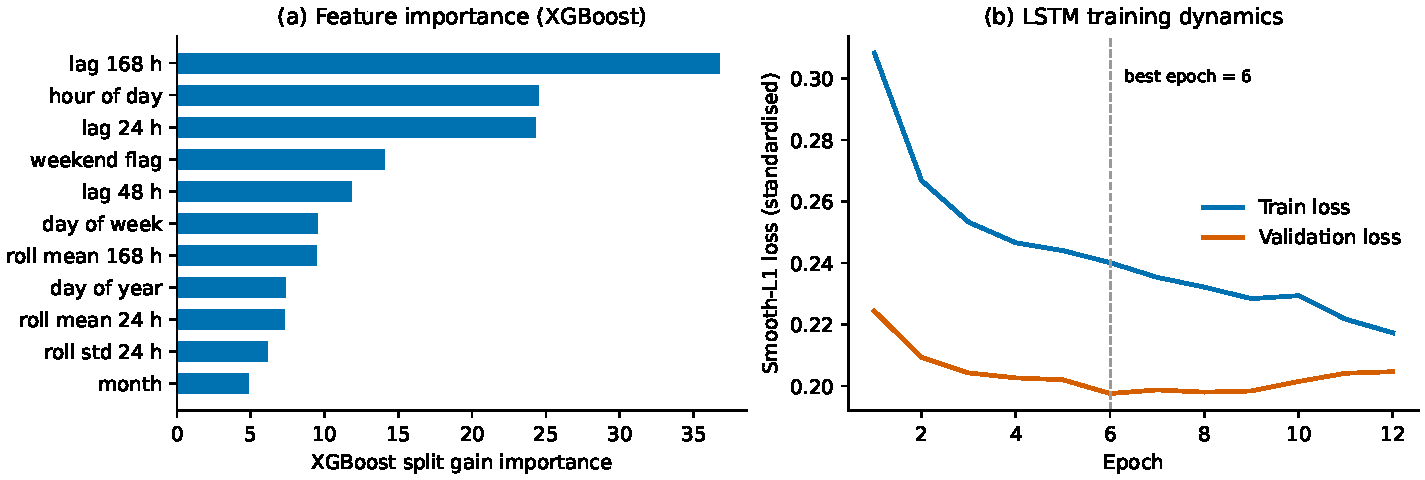
\includegraphics[width=0.9\textwidth]{../figures/fig5_importance_lstm.pdf}
\caption{Model diagnostics. (a) XGBoost split-gain feature importance: the
previous day's same-hour value and weekly structure dominate, with rolling means
providing local level; (b) LSTM training and validation loss (standardised
Smooth-$L_1$) with early stopping at the best validation epoch.}
\label{fig:importance}
\end{figure}

Figure~\ref{fig:importance}(a) ranks XGBoost features by split gain. The 24-hour lag
is the single most used split, followed by the 168-hour lag and the 24-hour rolling
mean---a compact confirmation that the model's predictive power comes from daily and
weekly persistence around an adaptive local level, with calendar features supplying
the remaining structure. Panel (b) shows the LSTM converged within six epochs and
began overfitting shortly after; early stopping on the validation split was
essential.

\subsection{Anomaly detection}
Table~\ref{tab:anomaly} reports the injected-anomaly benchmark and
Figure~\ref{fig:anomaly} visualises the trade-offs.

\begin{table}[t]
\centering
\caption{Anomaly detection on the injection benchmark (112 anomalous hours,
2.02\% of test; operating point set to true prevalence). Best value per column in
bold.}
\label{tab:anomaly}
\footnotesize
\begin{tabular*}{\textwidth}{@{\extracolsep{\fill}} l r r r r r r r r}
\toprule
 & & & & & & \multicolumn{3}{c}{\textbf{Recall by type}} \\
\cmidrule(lr){7-9}
\textbf{Detector} & \textbf{Prec.} & \textbf{Recall} & \textbf{F1} &
\textbf{ROC-AUC} & \textbf{PR-AUC} & \textbf{Spike} & \textbf{Shift} &
\textbf{Drop.} \\
\midrule
Residual z-score (XGB) & \textbf{0.482} & \textbf{0.482} & \textbf{0.482} &
\textbf{0.885} & \textbf{0.488} & \textbf{0.932} & \textbf{0.333} & \textbf{0.057} \\
LSTM-AE               & 0.402 & 0.402 & 0.402 & 0.721 & 0.314 & 0.977 & 0.061 & 0.000 \\
One-Class SVM          & 0.232 & 0.232 & 0.232 & 0.726 & 0.130 & 0.523 & 0.091 & 0.000 \\
Isolation Forest       & 0.196 & 0.196 & 0.196 & 0.731 & 0.114 & 0.409 & 0.121 & 0.000 \\
\bottomrule
\end{tabular*}
\end{table}

\begin{figure}[t]
\centering
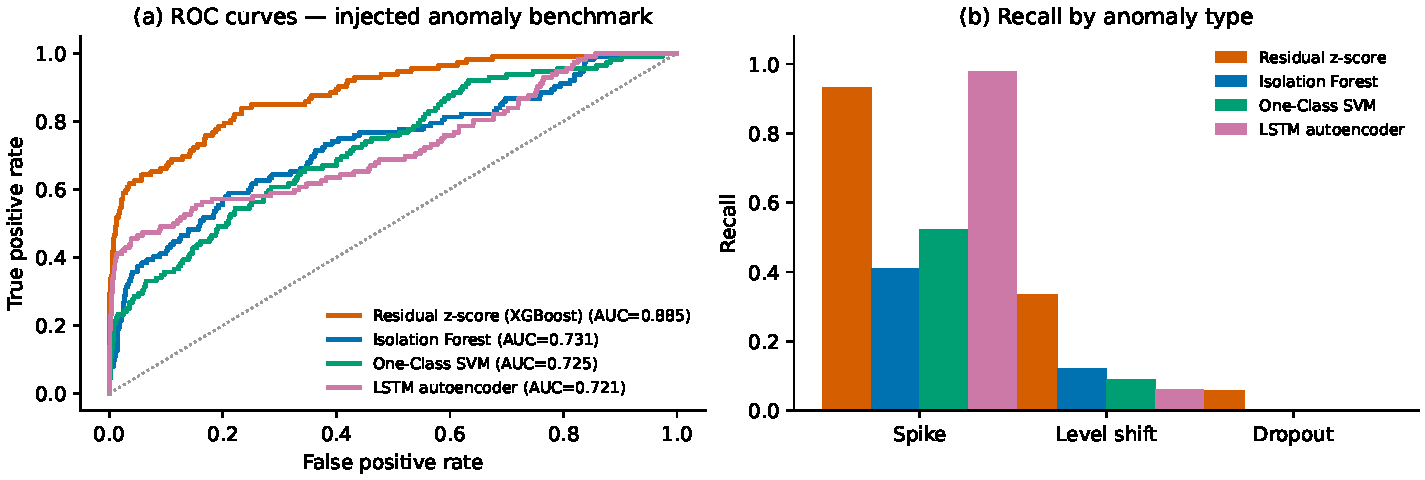
\includegraphics[width=0.9\textwidth]{../figures/fig6_anomaly_results.pdf}
\caption{Anomaly detection benchmark. (a) ROC curves of the four detectors on the
injection test; (b) recall decomposed by anomaly type, exposing the spike--dropout
asymmetry: spikes are near-certainly detected, dropouts almost never.}
\label{fig:anomaly}
\end{figure}

The \textbf{residual z-score is the strongest detector overall} (ROC-AUC 0.885,
F1 0.482), and it is the only method with non-zero recall on every anomaly type. Its
advantage is structural: the XGBoost forecaster contextualises each hour against
calendar and persistence features, so the residual isolates deviations from
\emph{expected} consumption rather than from the global feature distribution.
A fixed 3-sigma threshold performs nearly identically (F1 0.469), so the operating
point is not sensitive in this regime.

The \textbf{per-type decomposition is the most instructive result}. Spikes---sudden
single-hour excesses---are detected almost perfectly by the two learned models
(93--98\% recall) and by half of the SVM decisions. Level shifts are detected only by
the residual method (33\%), which notices the sustained gap between actual and
predicted level, while window-based methods average the anomaly away. Dropouts
(near-zero blocks mimicking vacancy or disconnection) escape \emph{all} detectors
(0--6\% recall): a 0.05\,kW reading is statistically indistinguishable from a normal
night hour when the local baseline is only 0.3--0.8\,kW, and the absolute residual
falls well inside three validation sigmas. Detecting low-side anomalies therefore
requires relative or asymmetry-aware scores, which we identify as the clearest
direction for future work.

The unsupervised feature-space methods (Isolation Forest, One-Class SVM) cluster in
the 0.72--0.73 ROC-AUC band: their scores respond to feature-space isolation, which
the contaminated lag features partially camouflage. The LSTM autoencoder reaches
0.402 F1 thanks to excellent spike recall but contributes nothing on sustained
anomalies under our point-wise localisation.

\subsection{Case study: real anomalies}
Applied to the clean test period, the residual detector flags 55 hours (0.99\%)
beyond three sigmas. Table~\ref{tab:casestudy} lists the strongest merged events;
Figure~\ref{fig:casestudy}(a) shows one week of detections and panel (b) the
detector operating against injected anomalies with its score trace.

\begin{table}[t]
\centering
\caption{Strongest anomaly events detected on the unmodified test period
(consecutive flagged hours merged; events within two hours joined).}
\label{tab:casestudy}
\small
\begin{tabular*}{\textwidth}{@{\extracolsep{\fill}} l l r r r r}
\toprule
\textbf{Start} & \textbf{End} & \textbf{Hours} & \textbf{Max $|z|$} &
\textbf{Actual (kW)} & \textbf{Forecast (kW)} \\
\midrule
2010-11-20 18:00 & 2010-11-20 18:00 & 1 & 5.2 & 5.63 & 2.31 \\
2010-11-04 08:00 & 2010-11-04 11:00 & 4 & 5.1 & 4.42 & 1.17 \\
2010-11-04 19:00 & 2010-11-04 20:00 & 2 & 4.7 & 4.46 & 1.49 \\
2010-07-01 00:00 & 2010-07-01 00:00 & 1 & 4.5 & 3.33 & 0.45 \\
2010-10-18 09:00 & 2010-10-18 19:00 & 5 & 4.5 & 3.84 & 0.99 \\
2010-05-15 23:00 & 2010-05-15 23:00 & 1 & 4.0 & 3.82 & 1.32 \\
\bottomrule
\end{tabular*}
\end{table}

\begin{figure}[t]
\centering
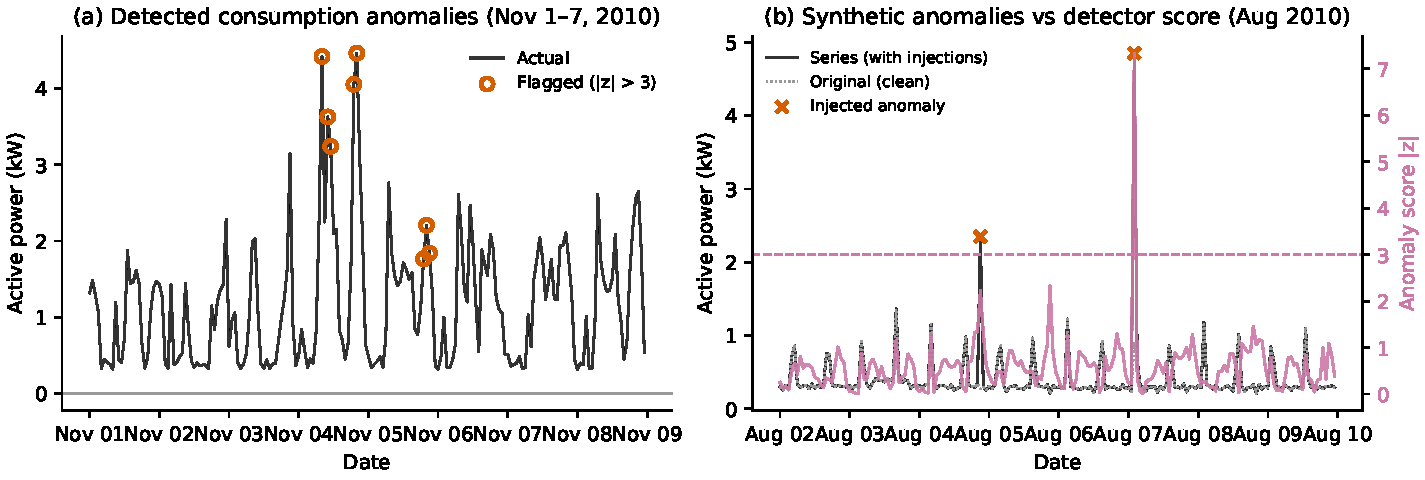
\includegraphics[width=0.9\textwidth]{../figures/fig7_anomaly_casestudy.pdf}
\caption{(a) Detected consumption anomalies (|z| $>$ 3, circled) during a clean test
week; (b) the detector score (right axis, purple) tracking injected anomalies
(crosses) in a synthetic window, with the 3-sigma decision threshold dashed.}
\label{fig:casestudy}
\end{figure}

The events are behaviourally plausible: single late-evening surges of 5--6\,kW
(consistent with high-wattage appliances or guests), and one remarkable
\emph{morning} excursion on 4 November 2010 in which consumption ran above 4\,kW for
four hours against a forecast of 1.2\,kW. All top events are high-side deviations,
mirroring the benchmark finding that the absolute-residual detector is
asymmetrically sensitive to excess consumption.

% ============================================================ 6
\section{Deployed Web System}\label{sec:web}

To close the gap between benchmark and practice, the selected XGBoost forecaster and
the residual anomaly detector are packaged as a Flask service
(Figure~\ref{fig:web}). The dashboard offers four views: a \emph{forecast} tab that
backtests any day of the test period---showing the preceding week of actual
consumption, the day-ahead forecast, and a $\pm1.96\sigma$ prediction band---and
accepts user-supplied hourly histories for genuine live forecasts; an
\emph{anomalies} tab that plots consumption, z-scores, and flagged hours for any
week, alongside the strongest real events; a \emph{models} tab rendering both
leaderboards; and an \emph{API} tab documenting the REST interface. The API exposes
\texttt{GET /api/forecast?date=}, \texttt{POST /api/forecast} for live inference
(minimum 216 hourly values; the model recursively consumes its own predictions
beyond the first horizon), \texttt{GET /api/anomaly?start=\&end=},
\texttt{GET /api/history}, \texttt{GET /api/models}, and
\texttt{GET /api/anomaly/casestudy}, all returning JSON.

Engineering choices target the Render free tier (512\,MB RAM): the service loads
only the 0.8\,MB XGBoost artefact plus pre-aggregated hourly data (3.9\,MB) and
residual scores, uses gunicorn with a single worker and four threads, and
deliberately excludes deep-learning runtimes, which would inflate the image by two
orders of magnitude for marginal accuracy gain. Every request after cold start is
served from memory; a live 24-hour forecast adds only recursive feature construction
and 24 tree traversals. A \texttt{render.yaml} blueprint, pinned requirements, and a
health check (\texttt{/api/health}) make deployment a one-click operation from the
public repository.

\begin{figure}[t]
\centering
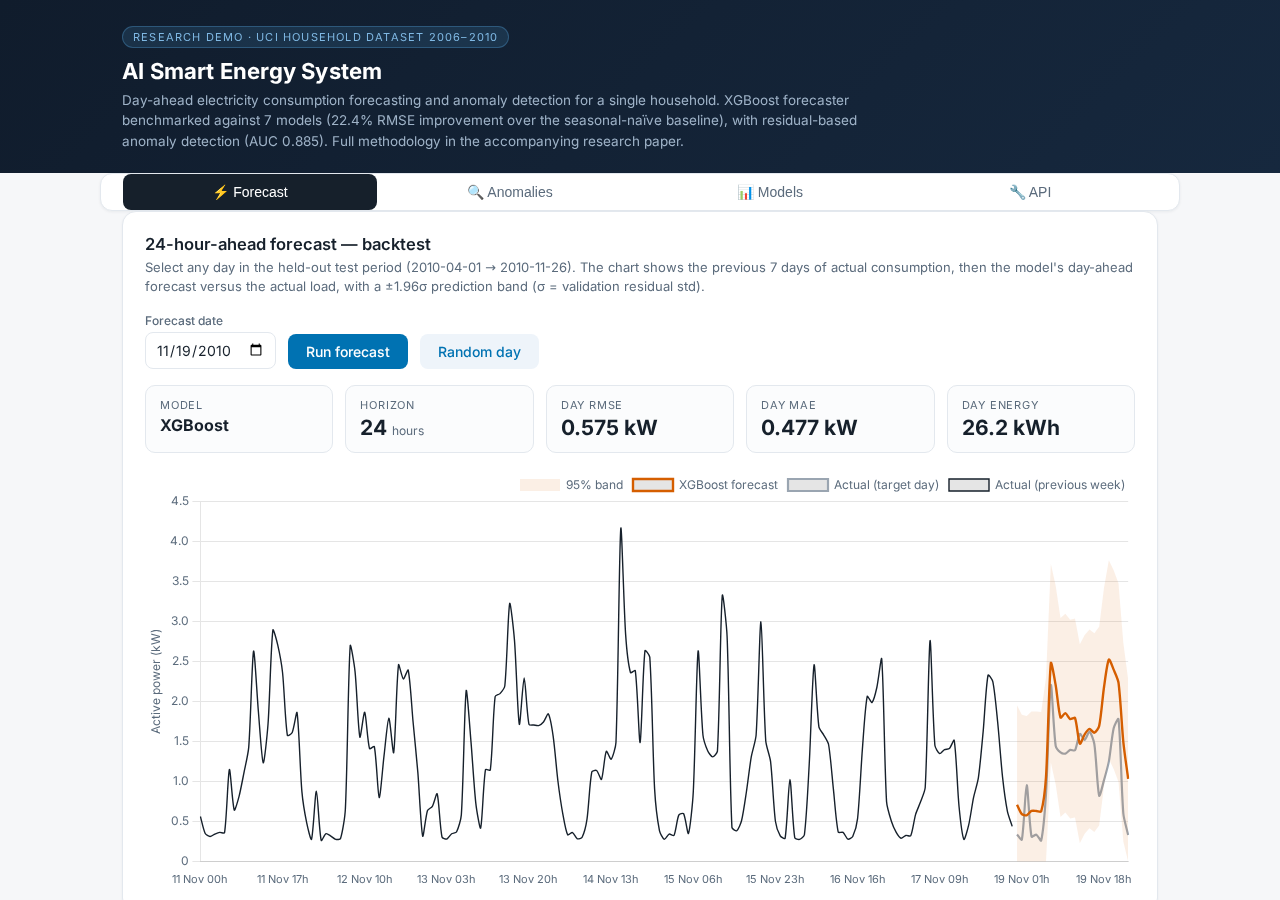
\includegraphics[width=0.8\textwidth]{../figures/web_forecast.png}
\caption{The deployed dashboard (local instance): day-ahead forecast backtest with
prediction band, day-level metrics, and navigation to the anomaly, leaderboard, and
API views.}
\label{fig:web}
\end{figure}

% ============================================================ 7
\section{Discussion and Limitations}\label{sec:discussion}

\textbf{Predictability ceiling.} The clustering of all learned models within a
1\% RMSE band, far above the na\"ive baselines but far below aggregate-load
accuracy, suggests the remaining error is dominated by irreducible occupant
stochasticity rather than model capacity. In this regime, model choice should be
driven by operational criteria---fit time, artefact size, inference latency---which
favours gradient-boosted trees for embedded and edge deployment.

\textbf{Asymmetric detectability.} The near-perfect spike recall versus
near-zero dropout recall is the sharpest finding of the anomaly study. It implies
that systems built on absolute forecast residuals will reliably catch excessive
consumption (often the financially significant failures: heaters left on, faulty
appliances) but will miss vacancy and disconnection events. Relative or
prediction-conditional scoring, and detectors that model the lower tail of the
consumption distribution explicitly, are promising remedies.

\textbf{Single household, synthetic anomalies.} All results derive from one meter in
one climate, and the injected anomalies are statistically simpler than real faults:
injection is a necessity on an unlabelled dataset. The methodology transfers
directly---features, protocol, and deployment are household-agnostic---but absolute
accuracies will differ with appliance mix, occupancy patterns, and climate, and
labelled field data would be required for definitive claims.

% ============================================================ 8
\section{Conclusion}\label{sec:conclusion}

We presented a complete, reproducible study of AI-based consumption prediction and
anomaly detection for a single household, spanning data engineering, an
eight-model day-ahead forecasting benchmark, a contamination-aware four-detector
anomaly evaluation, error and failure analysis, and a deployed web system. Gradient
boosting (XGBoost) delivered the best test RMSE (0.588\,kW, 22.4\% skill over the
seasonal na\"ive), with an LSTM competitive and best on MAE/MAPE; forecast-residual
z-scoring dominated anomaly detection (ROC-AUC 0.885), and the per-type analysis
revealed a fundamental spike--dropout asymmetry that defines the open problem for
low-side anomaly detection. The accompanying repository releases all code, trained
models, figures, the research paper, a Kaggle training notebook, and a one-click
Render deployment, so that both the results and the running system can be
independently verified and extended.

% ============================================================ refs
\setlength{\bibsep}{1.5pt plus 1pt}
\renewcommand{\bibfont}{\footnotesize}
\bibliography{refs}

\end{document}
